\documentclass{article} \usepackage{amsmath} \usepackage{amssymb} \usepackage{amsthm} \usepackage[margin=0.2in]{geometry} \usepackage{hyperref} \usepackage{physics} \usepackage{tikz} \usepackage{mathtools} \mathtoolsset{showonlyrefs} \theoremstyle{definition} \newtheorem{theorem}{Theorem}[section] \newtheorem{corollary}{Corollary}[theorem] \newtheorem{lemma}[theorem]{Lemma} \newtheorem{definition}{Definition}[section] \author{Connor Duncan} \date{\today}
\title{Physics-105-Lecture-Notes-04-18-2019}
\begin{document}
\maketitle\tableofcontents
\noindent\abstract{A single PDF with all lectures in a single document can be downloaded at \url{https://www.dropbox.com/sh/8sqzvxghvbjifco/AAC9LoSRnsRQDp7pYedgWpQMa?dl=0}. The password is 'analytic.mech.dsp'.
 This file was automatically generated using a script, so there might be some errors. If there are, you can contact me at \url{mailto:ctdunc@berkeley.edu}.}
Lagrangian density for some discrete masses on string, with $y_k$ change in $y$, and $\eta_k$ displacement in $x$, then \begin{equation} \mathcal L = \frac{1}{2}\rho(x)\left(\pdv{y}{t}\right)^2-\frac{1}{2}\tau(x)\left(\pdv{y}{x}\right)^2+O(\eta) \end{equation} where $O(\eta)$ higher order terms Recall our equation of motion \begin{equation} \pdv{x}\left(\tau(x)\pdv{y}{x}\right)=\rho(x)\pdv[2]{y}{t} \end{equation} if we require $\tau$ constant, then we get $\pdv[2]{y}{x}=\frac{1}{c(x)}\pdv[2]{y}{t}$. \section{Solving the Wave Equation} Two methods of solving \begin{itemize} \item Computer \item Pertubation Theory (only valid for $\lambda\ll[\dv{x}(\ln(l''_s))]^{-1}$ or $\lambda\ll\frac{1}{\frac{1}{c_s}\dv{L_s}{x}}$. Often called the WKB approximation. Basically $\lambda$ is less than the second $x$ derivative of a typical length scale. GOOGLE. \end{itemize} Let's take the following new variables, \begin{align} \xi=x-vt \\ \eta=x+vt \end{align} so that $(x,t)\rightarrow(\xi,\eta)$. So, we now have \begin{align} \pdv{y}{x}=\left(\pdv{\xi}+\pdv{\eta}\right)y \\ \pdv[2]{y}{x}=\left(\pdv[2]{\xi}+2\pdv[2]{}{\xi}{\eta}+\pdv[2]{\eta}\right)y \\ \pdv{y}{t}=c_s\left(\pdv{\eta}-\pdv{\xi}\right)y \\ \pdv[2]{y}{t}=c_s^2\left(c_s\pdv[2]{\xi}-2\pdv[2]{}{\eta}{\xi}+\pdv[2]{\eta}\right)y \end{align} so we can find some solution by setting \begin{equation} y(x,t)=f(x-c_st)+g(x+c_st) \end{equation} if we set $g\equiv 0$, then \begin{align} y(x,t)=f(x-c_st) && y(x,0)=f(x) \end{align} \begin{center} \begin{tikzpicture}[scale=2] \draw[->] (0,0.5)--(0.3,0.5); \draw (-1,1) -- (-0.2,1) sin (0,1.3) cos (0.2,1) -- (1,1); \draw (-1,0) -- (0,0) sin (0.2,0.3) cos (0.4,0) -- (1,0); \draw[dashed] (0,-.2) -- (0,1.4); \draw[dashed] (0.2,-.2)--(0.2,1.4); \draw[<->] (0,-.2)--(0.2,-.2); \node (label) at (0.1,-.4) {$c_s\Delta t$}; \end{tikzpicture} \end{center} traveling wave solution, it only goes from $x\rightarrow x+c_s\Delta t$. In the arbitrary solution, we have \begin{align} y(x,t)=f(x-ct)+g(x+ct) \end{align} where $f,g$ are determined by initial conditions. (i.e. at $t=0$, we have $f(x)+g(x)=y_0(x)$). taking \begin{equation} \pdv{g}{x}-\pdv{f}{x}=\frac{1}{c_s}\dot y_0(x) \end{equation} we integrate to see that \begin{equation} g(x)-f(x)=\frac{1}{c_s}\int_{x_0}^x\dot y_0(x')dx' \end{equation} which gives \begin{align} f(x)=y_0(x)=\frac{1}{c}\int_{x_0}^x\dot y_0(x')dx' \\ g(x)=y_0(x)+\frac{1}{c}\int_{x_0}^x\dot y_0(x')dx' \end{align} Then, we also have \begin{equation} y(0,t)=f(x-ct)+g(x+ct) \end{equation} so we can write the D'lambert solution to the wave equation. \begin{equation} y(x,t)=\frac{1}{2}\left[y_0(x-ct)+y_0(x+ct)\right]+\frac{1}{2c}\int_{x-ct}^{x+ct}\dot y_0(x')dx' \end{equation} for a small pertubation, the solution of this immediately becomes that there are two pulses \begin{center} 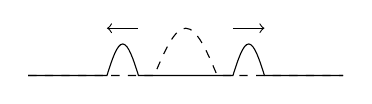
\begin{tikzpicture}[scale=2] \draw (-1,0) -- (-0.5,0) sin (-0.4,0.2) cos (-0.3,0) -- (0.3,0) sin (0.4,0.2) cos (0.5, 0) -- (1,0); \draw[dashed] (-1,0) -- (-0.2,0) sin (0.0,0.3) cos (0.2,0) -- (1,0); \draw[<-] (-0.5,0.3)--(-0.3,0.3);\draw[->](0.3,0.3)--(0.5,0.3); \end{tikzpicture} \end{center} propagating in opposite directions. \subsection{General Solution} The generalized wave equation can be written \begin{equation} \nabla^2\psi=\frac{1}{c^2}\pdv[2]{\psi}{t} \end{equation} There are several categories of solutions to consider. First is a standing wave, $\psi(\vec{r},t)$ depends as $A(\vec{r})e^{-i\omega t}$. We get the \textbf{Helmholtz Equation} that describes such solutions. \begin{align} \nabla^2A(r)+\frac{\omega^2}{c^2}A(\vec{r})=0 \end{align} The 1-d case (say for a string with fixed boundaries is given as \begin{equation} \pdv[2]{A}{x}+\frac{\omega^2}{c^2}A=0 \end{equation} so given that $A(0)=A(L)=0$, then the boundary condition for the left gives $A(x)=a\sin(\frac{\omega}{c}x)$. We also need $\sin(\frac{\omega}{c}L)=0$, then possible frequencies given $\Omega=\{\frac{c\pi n}{L}|n\in\mathbb{Z}\}$. So, the general solution is written \begin{equation} \psi_n(x,t)=e^{-i\omega_n t}\sin(\frac{\pi n}{L}x) \end{equation} with $\omega_n=\frac{\pi n }{L}c$. Fun math fact, we can write down the general solution for one dimension as \begin{equation} \psi(x,t)=\sum_{n=1}^\infty[a_n\cos(\omega_n)t+b_n\sin(\omega_n t)]\times \sin\frac{\pi n}{L}x \end{equation} if you do the math out you get thatt \begin{align} a_n=\frac{2}{L}\int_0^L\psi(x,0)\sin(\frac{\pi n}{L}x)dx \\ \omega_nb_n=\frac{2}{L}\int_0^L\pdv{\psi}{t}\sin\frac{\pi}{n}Ldx \end{align} \subsection{2-d Helmholz} \begin{equation} \psi=e^{-i\omega t}A(x,y) \end{equation} Say some membrane, with $\psi$ some oscillation in $z$ over a bounded membrane \begin{center} \begin{tikzpicture}[scale=2] \draw[->] (0,0)--(0,1) node[anchor=east] {$y$}; \draw[->] (0,0)--(1,0) node[anchor=west] {$x$}; \draw[dashed] (0,0) rectangle (0.5,0.5) ; \end{tikzpicture} \end{center} Let's take \begin{equation} \left(\pdv[2]{x}+\pdv[2]{y}+\frac{\omega^2}{c^2}\right)A=0 \end{equation} under teh assumption that $A$ is separable, i.e. $A=X(x)Y(y)$. Then we can write \begin{equation} X''(x)Y(y)+Y''(y)X(x)+\frac{\omega^2}{c^2}XY=0 \end{equation} which, we can divide by $XY$ to get \begin{equation} \frac{X''}{X}+\frac{Y''}{Y}+\frac{\omega^2}{c^2}=0 \end{equation} so, let's write some stuff down \begin{align} X''(x)=-\lambda X, && \lambda\equiv\text{const}\\ Y''(y)=-\mu Y && \mu\equiv\text{const} \end{align} we have the boundary conditions that $X=a\sin(\sqrt{\lambda}x)$, also with $\sin(\sqrt{\lambda} L)=0$, so we have \begin{align} X_n(x)=a\sin\left(\frac{\pi n}{L}x\right) \\ Y_m(y)=b\sin\left(\frac{\pi m}{L}y\right) \end{align} we also know that \begin{equation} \frac{\omega^2}{c^2}(\lambda+\mu)\Rightarrow\frac{\omega_{nm}^2}{c^2}=\frac{\pi^2(n^2+m^2)}{L^2} \end{equation} which gives some general solution \begin{equation} \psi(x,y,t)=\sum_{n=1}^\infty\sum_{m=1}^\infty(a_{nm}\cos(\omega_{nm}t)+b_{nm}\sin(\omega_{nm}t))X_n(x)Y_m(y) \end{equation} \subsubsection{Circular Boundary} If we have some circular boundary, we still have the same helmholz, and $A=A(r,\theta)$. We rewrite the laplacian in cylindciral coordinates and get \begin{equation} \frac{1}{r}\dv{r}\left(r\pdv{A}{r}\right)+\frac{1}{r^2}\pdv[2]{A}{\theta}+\frac{\omega^2}{c^2}A=0 \end{equation} Apply condition $A(r,0)=A(r,2\pi R_0)$, and $A(r,\theta)=R(r)e^{-im\theta}$. \subsubsection{Bessel function} \begin{equation} y''(x)+\frac{1}{x}y'(x)+\left(\lambda^2-\frac{n^2}{x^2}\right)y=0 \end{equation} so that the \emph{Bessel Functions} of order $n$ are given as solutions to this bad boy. \begin{equation} y(x)=J_n(\lambda x) \end{equation} We have \begin{equation} R''(r)+\frac{1}{r}R'(r)+\left(\frac{\omega^2}{c^2}-\frac{m^2}{r^2}\right)R=0 \end{equation} which gives solution \begin{equation} R=J_m(\frac{\omega}{c}r) \end{equation} we apply that it must satisfy the boundary condition $J_m(\frac{\omega}{c_s}R_0=0$, which give solutions. I don't think it's gonna be super important to know how to solve this, but basically it;s the roots of the bessel function (this is the wave equation for a spherically propagating wave, which is how the double slit experiment works!). so the full on solutions are given as \begin{equation} \psi=J_m\left(\frac{\omega_{nm}}{c}\right) \times\left\{ \begin{matrix} \cos(m\varphi) \\ \sin(m\varphi) \end{matrix} \right\}\times \times e^{-i\omega_{nm}t} \end{equation} If we consider the case for oscillaating membranes on a cylinder, we'd write down \begin{equation} \frac{1}{r}\pdv{r}\left(r\pdv{A}{r}\right)+\frac{1}{r^2}\pdv[r]{A}{\theta}+\pdv[2]{A}{z}+\frac{\omega^2}{c^2}A=0 \end{equation} which becomes, with $A=R(r)Z(z)e^{-im\theta}$ \begin{equation} \frac{1}{Rr}\pdv{r}\left(r\pdv{A}{r}\right)-\frac{m^2}{r^2}+\frac{Z''(z)}{Z}+\frac{\omega^2}{c^2}=0 \end{equation} we just get anotherr \begin{equation} Z''(z)+\lambda Z(z)=0 \end{equation} which gives solutions of the bessel equation with differend conditions, we fund \begin{equation} R''+\frac{1}{r}R'-\frac{m^2}{r^2}R+\left(\frac{\omega^2}{c^2}-\left(\frac{\pi n}{L}\right)^2\right)R=0 \end{equation} which reduces \begin{align} R''+\frac{1}{r}R'+\left(\frac{\omega^2}{c^2}-\left(\frac{\pi n}{L}\right)^2-\frac{m^2}{r^2}\right)R=0 \\ R(r)=J_k(\sqrt{\frac{\omega^2}{c^2}-\left(\frac{\pi n}{L}\right)}r) \end{align}
\end{document}
